\documentclass[11pt]{article}

% ---------------------------------------------------------------- packages
\usepackage[margin=1.05in]{geometry}
\usepackage[utf8]{inputenc}
\usepackage[T1]{fontenc}
\usepackage{lmodern}
\usepackage{microtype}
\usepackage{amsmath,amssymb,amsthm,mathtools}
\usepackage{booktabs,array,multirow}
\usepackage{xcolor}
\usepackage{algorithm}
\usepackage{algpseudocode}
\usepackage{tikz}
\usetikzlibrary{positioning,arrows.meta,shapes.geometric,calc,fit,backgrounds}
\usepackage{pgfplots}
\pgfplotsset{compat=1.17}
\usepackage[numbers,sort&compress]{natbib}
\usepackage[hidelinks]{hyperref}
\usepackage[capitalise]{cleveref}
\makeatletter\def\theHALG@line{\thealgorithm.\arabic{ALG@line}}\makeatother

% ---------------------------------------------------------------- macros
\newcommand{\F}{{\mathbb{F}_2}}
\newcommand{\MM}[3]{\langle #1,#2,#3\rangle}
\newcommand{\rk}{\operatorname{rk}}
\newcommand{\supp}{\operatorname{supp}}
\newcommand{\bits}{\operatorname{bits}}
\newcommand{\tensor}{\otimes}
\newcommand{\file}[1]{\texttt{#1}}
\newcommand{\todo}[1]{{\color{red}[TODO: #1]}}

\theoremstyle{plain}
\newtheorem{lemma}{Lemma}
\newtheorem{proposition}{Proposition}
\theoremstyle{definition}
\newtheorem{definition}{Definition}

\Crefname{algorithm}{Algorithm}{Algorithms}

% ---------------------------------------------------------------- front matter
\title{Directed Flip-Graph Walks, Projection Cascades and\\
Composition Closure for GF(2) Matrix-Multiplication Schemes:\\
Search Methods with Provenance-Preserving Verification}
\author{Erik Peterson\thanks{\todo{affiliation and contact e-mail}}}
\date{\today\ \textbf{(draft)}}

\begin{document}
\maketitle

\begin{abstract}
Upper bounds on the tensor rank of matrix multiplication over $\F$ are found by random walks on flip graphs and by composing known schemes.
We describe the pipeline behind a large 2026 campaign, whose outcome is reported in a companion paper: a single-threaded, allocation-free \emph{directed} flip-graph walker with bit-packed multiword factors, whose walks replay byte for byte, on the same build, from a seed file, a step count and a nonce; a cross-shape derivation step that projects a scheme onto a smaller shape after a shared-factor basis rewrite; a rank-only composition closure over block sums and Kronecker products, materialized into witnesses; ingestion of public integer and ternary schemes modulo two, and replay of matmulcatalog derivations over $\F$; a scoring discipline against four public rank tables; and \emph{lineage bundles} whose tensors are checked by two separately written exactness verifiers and whose seed, projection and replay rows are re-derived from pinned upstream revisions.
Over 4{,}816 walks (\(3.1\times10^{11}\) proposals) the stages differ by orders of magnitude in yield: 40M-move walks from projection children lowered the rank below their starting rank in 90\% of cases (relative to unreduced seeds, so not a yield of records), against 0.95\% for walks from public integer schemes.
We report a reproducibility defect that only a verification from a clean extraction with empty caches exposed, and comparison pitfalls: a comparison with the four tables alone overstated novelty, since a later check found 87 of 795 results superseded by published constructions or rank claims (80 rebuilt and verified, 7 claims) and 112 more matched by compositions of published schemes or claims.
Every claim is an upper bound; nothing here proves optimality.
\end{abstract}

\noindent\textbf{Keywords:} matrix multiplication, tensor rank, bilinear algorithms, flip graphs,
$\mathrm{GF}(2)$, exact verification, reproducibility.\\
\textbf{MSC 2020:} 68Q25, 15A69, 68W30. \quad \textbf{ACM CCS:} Computing methodologies $\to$ Symbolic and algebraic algorithms.

\section{Introduction}\label{sec:intro}

A scheme of rank $r$ for $n\times m$ by $m\times p$ matrix multiplication computes the product with $r$
non-commutative multiplications of linear forms; equivalently it writes the matrix-multiplication
tensor $\MM nmp$ as a sum of $r$ rank-one tensors \cite{burgisser1997algebraic,landsberg2012tensors,blaser2013fast}.
Since Strassen's rank-7 scheme for $\MM222$ \cite{strassen1969gaussian}, upper bounds for small formats have come from
clever constructions \cite{hopcroft1971minimizing,laderman1976noncommutative,smirnov2013bilinear}, from
SAT and local search \cite{heule2019local,heule2021new}, from reinforcement learning \cite{fawzi2022discovering}, from
program evolution \cite{novikov2025alphaevolve} and, most productively in recent years, from random walks on \emph{flip graphs}
\cite{kauers2023flip,arai2024adaptive,moosbauer2025flip,kauers2025meta,perminov2025ternary}.
The field matters: over $\F$ there are schemes that do not exist in other characteristics.
The best-known example is the rank-47 scheme for $\MM444$ \cite{fawzi2022discovering}; for $\MM555$ the $\F$ record
went $98\to96\to95\to94\to93$ \cite{sedoglavic2021tensor,fawzi2022discovering,kauers2022still,arai2024adaptive,moosbauer2025flip}.

Best-known ranks for all formats up to $32\times32\times32$ are collected in two public tables
\cite{sedoglavic2026catalogue,lacelle2026catalog}; two repositories hold explicit schemes for the formats up to $16\times16\times16$
\cite{perminov2026fmmrepo} and for 25 formats \cite{witteveen2026schemes}.
Small formats are the subject of intense search.
Large formats mostly are not searched at all: the listed ranks there come from composing smaller
schemes by block sums and Kronecker products, so they respond to any improvement of a component,
and the components that matter in characteristic two (the rank-47 scheme above, in particular) are
not the ones the general-ring tables were built from.

This paper describes a pipeline that attacks that regime and the engineering needed to make its
output believable.
It was used for a campaign in September 2026. The results, pooled from three stages of the project (July, 2026-09-22 to 09-26,
and the campaign of 2026-09-26 to 09-29), are 795 shapes for which our best verified scheme is below every GF(2)-valid rank listed in four public tables at the pinned revisions
(733 of them also below every rank listed in any ring); they are reported in a companion paper \cite{peterson2026results}.
Here we concentrate on \emph{how} the schemes were obtained, how they were checked, and what each stage of the campaign was worth.
The campaign ran 4{,}816 walks totalling \(3.1\times10^{11}\) proposals over 2{,}708 distinct shapes,
materialized 942 composition products, replayed 1{,}352 derivation recipes from the matmulcatalog (1{,}098 of them exactly over $\F$),
and verified every tensor that is claimed.

\paragraph{Contributions.}
\begin{enumerate}
\item A \textbf{directed flip-graph walker} for formats with all sides at least 2 and factors of up to $1{,}024$ bits
(\cref{sec:walker}): proposals are sampled only among factor buckets that contain a flippable pair,
factors are multiword bit vectors, memory is allocated once, and a walk is a deterministic function of
(seed file, number of proposals, nonce). We report its per-proposal cost as a function of factor width
and the byte-for-byte replay of 42 distinct campaign walks.
\item A \textbf{cross-shape derivation step} (\cref{sec:derive}): coordinate deletion applied to the best
scheme after a shared-factor basis rewrite, followed by shared-factor compression. Walks from these
``projection children'' lowered the rank below the child's own starting rank in 792 of 880 cases, at 44M proposals per
lowering against 0.3--9G for the seed classes that do not descend from projection children (0.16G for the deepening of projection lineages); children start unreduced, so this measures the slack that projection
leaves for the walker rather than the yield of records.
\item A \textbf{rank-only composition closure} with witness-backed materialization (\cref{sec:composition}):
a dynamic programme over all 5{,}984 sorted formats with sides $\le32$ that prices block sums and Kronecker products in
0.3\,s, followed by construction and exact checking of each priced improvement.
\item \textbf{Seeds from public tables} (\cref{sec:seeds}): reduction of published ternary and integer schemes
modulo two behind a ring gate, and replay of matmulcatalog derivation recipes over $\F$, including detection of recipes whose
``F2'' stamp over-claims and a case study of a cache-history dependence that made replays
non-reproducible until it was fixed.
\item A \textbf{scoring and claim discipline} (\cref{sec:scoring}): what to compare against, which comparisons are
invalid (commutative algorithms, wrong ring, stale tables), and how field-agnostic tables distort the picture.
\item \textbf{Lineage bundles and a verification protocol} (\cref{sec:lineage}) in which every tensor is expanded against
the full matrix-multiplication tensor by two separately written implementations; projection, public-seed, archived and retained rows
are recomputed from their source; 42 of 244 distinct walks are replayed and 71 of 82 catalogue replays are reproduced from an empty cache;
and the check is repeated from a clean extraction.
\item An \textbf{empirical account of yield and cost} per stage, including the negative results (\cref{sec:eval}).
\end{enumerate}

\begin{figure}[t]
\centering
\resizebox{\textwidth}{!}{%
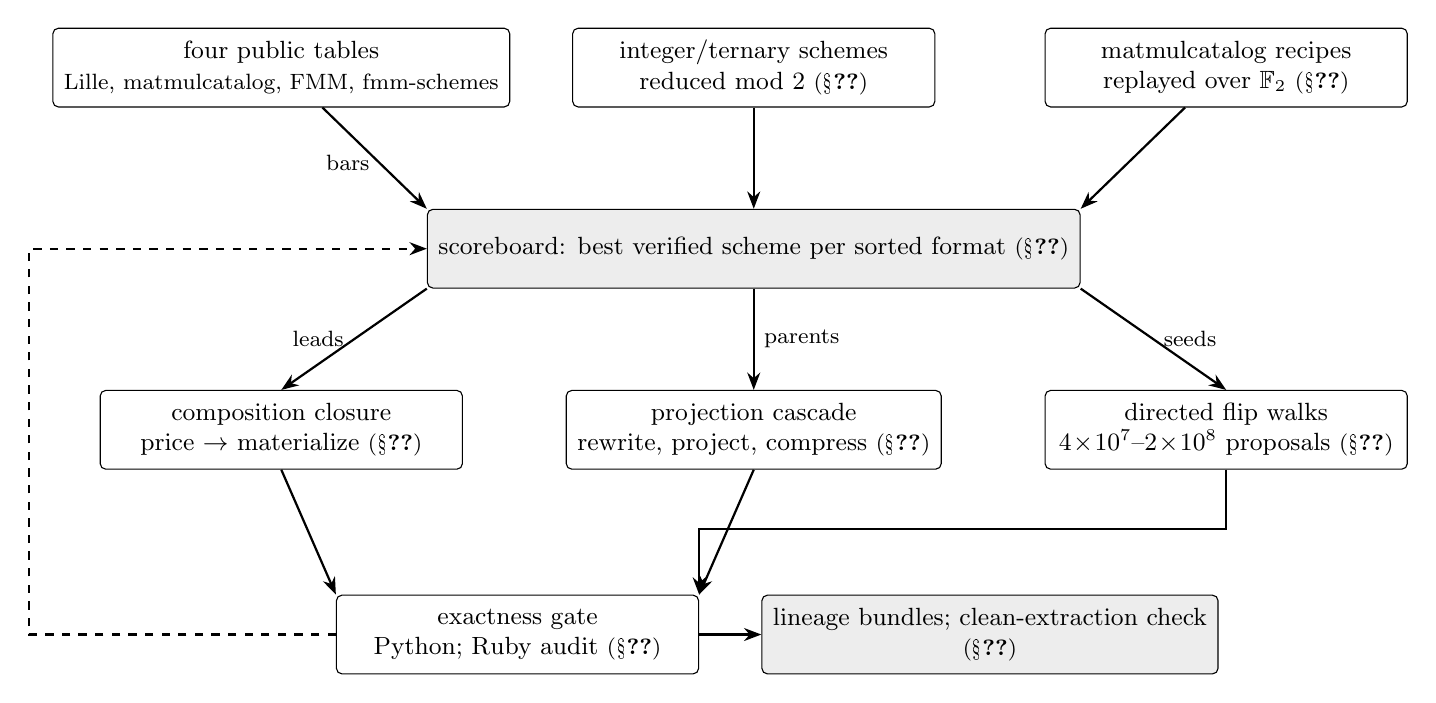
\begin{tikzpicture}[
  box/.style={draw,rounded corners=2pt,align=center,inner sep=4pt,font=\small,minimum height=10mm,minimum width=46mm},
  shade/.style={fill=gray!14},
  arr/.style={-{Stealth[length=2.2mm]},thick}]
  % sources
  \node[box] (tab) at (0,6.0) {four public tables\\ {\footnotesize Lille, matmulcatalog, FMM, fmm-schemes}};
  \node[box] (pub) at (6.0,6.0) {integer/ternary schemes\\ reduced mod 2 {\footnotesize(\S\ref{sec:seeds})}};
  \node[box] (rep) at (12.0,6.0) {matmulcatalog recipes\\ replayed over $\mathbb F_2$ {\footnotesize(\S\ref{sec:seeds})}};
  % scoreboard
  \node[box,shade,minimum width=76mm] (board) at (6.0,3.7) {scoreboard: best verified scheme per sorted format {\footnotesize(\S\ref{sec:scoring})}};
  % operators
  \node[box] (clo) at (0,1.4) {composition closure\\ price $\to$ materialize {\footnotesize(\S\ref{sec:composition})}};
  \node[box] (proj) at (6.0,1.4) {projection cascade\\ rewrite, project, compress {\footnotesize(\S\ref{sec:derive})}};
  \node[box] (walk) at (12.0,1.4) {directed flip walks\\ $4\!\times\!10^{7}$--$2\!\times\!10^{8}$ proposals {\footnotesize(\S\ref{sec:walker})}};
  % gate and bundle
  \node[box] (gate) at (3.0,-1.2) {exactness gate\\ Python; Ruby audit {\footnotesize(\S\ref{sec:repr})}};
  \node[box,shade] (bundle) at (9.0,-1.2) {lineage bundles; clean-extraction check\\ {\footnotesize(\S\ref{sec:lineage})}};
  \draw[arr] (tab) -- node[left,font=\footnotesize,pos=0.55]{bars} (board.north west);
  \draw[arr] (pub) -- (board.north);
  \draw[arr] (rep) -- (board.north east);
  \draw[arr] (board.south west) -- node[left,font=\footnotesize]{leads} (clo.north);
  \draw[arr] (board.south) -- node[right,font=\footnotesize]{parents} (proj.north);
  \draw[arr] (board.south east) -- node[right,font=\footnotesize]{seeds} (walk.north);
  \draw[arr] (clo.south) -- (gate.north west);
  \draw[arr] (proj.south) -- (gate.north east);
  \draw[arr] (walk.south) |- ++(0,-0.75) -| (gate.north east);
  \draw[arr] (gate) -- (bundle);
  \draw[arr,dashed] (gate.west) -- ++(-3.9,0) |- (board.west);
\end{tikzpicture}}
\caption{The pipeline. Every tensor enters the scoreboard only through the exactness gate (dashed arrow); the public tables steer effort (bars, leads, parents, seeds) but never admission.}
\label{fig:pipeline}
\end{figure}


\paragraph{What is not claimed.}
Projection, block composition and Kronecker products are classical; our contribution there is the
shared-factor basis rewrite before projection, the materialization from GF(2)-valid leaves and the measured yield, not a new mathematical operation.
Every rank reported anywhere is an upper bound. We prove no lower bounds, we do not claim optimality, and, following
the record policy of the project, results that beat a table are called \emph{apparent} until a complete prior-art
audit has been done (\cref{sec:scoring,sec:limits}).

\paragraph{Organization.}
\Cref{sec:background} fixes notation. \Cref{sec:repr} defines the scheme format and the exactness gate,
\cref{sec:walker} the walker, \cref{sec:derive} projection and basis rewriting, \cref{sec:composition} composition closure and
\cref{sec:seeds} the use of public schemes. \Cref{sec:scoring} covers scoring, \cref{sec:lineage} provenance and verification,
\cref{sec:eval} the campaign's measured behaviour and \cref{sec:limits} limitations.

\section{Background and notation}\label{sec:background}

\paragraph{Schemes.}
Index the entries of an $n\times m$ matrix $A$ by pairs $(i,j)$ and identify the pair with the coordinate $i\,m+j$
(row-major). Let $e_{(i,j)}$ be the corresponding standard basis vector of $\F^{nm}$. The matrix-multiplication tensor is
\[
  T_{n,m,p} \;=\; \sum_{i<n,\;j<m,\;k<p} e_{(i,j)}\tensor e_{(j,k)}\tensor e_{(i,k)}
  \;\in\; \F^{nm}\tensor\F^{mp}\tensor\F^{np}.
\]
Note that the third factor is indexed by the entry $(i,k)$ of the \emph{product}, not transposed.
A \emph{scheme of rank $r$ for $\MM nmp$ over $\F$} is a list of $r$ triples $(u_t,v_t,w_t)$ of nonzero vectors with
$\sum_t u_t\tensor v_t\tensor w_t = T_{n,m,p}$. Equivalently, for all $A\in\F^{n\times m}$ and $B\in\F^{m\times p}$,
\[
  (AB)_{ik} \;=\; \sum_{t=1}^{r} w_t[(i,k)]\;\langle u_t,A\rangle\,\langle v_t,B\rangle ,
\]
so the scheme computes the product with $r$ multiplications of linear forms in the entries of $A$ and $B$.
We write $\rk_{\F}\MM nmp$ for the least such $r$. Every scheme found by any of our tools is an \emph{upper bound}
for this quantity; we never certify a lower bound.

\paragraph{Orientation.}
The tensor $T_{n,m,p}$ is carried to $T_{m,p,n}$ and to $T_{p,m,n}$ by cyclic shifts of the three factors and by transposition of the
matrices, with the appropriate re-indexing of coordinates. Hence $\rk_{\F}\MM nmp$ depends only on the multiset $\{n,m,p\}$. All tables and
all price computations in this paper key on the \emph{sorted} shape, and a scheme found for one orientation is turned into a scheme for
another by an explicit coordinate permutation (with a transposition of a factor when the permuted edge is reversed) that is itself
covered by the exactness gate of \cref{sec:repr}.

\paragraph{Symmetries.}
The isotropy group $\mathrm{GL}_n(\F)\times\mathrm{GL}_m(\F)\times\mathrm{GL}_p(\F)$ acts on schemes for $\MM nmp$ and is the source of
the many equivalent presentations of a fixed scheme \cite{degroote1978isotropy,burichenko2015symmetries}.
The walker of \cref{sec:walker} does not use it; the derivation step of \cref{sec:derive} acts on presentations by a different mechanism
(refactoring the terms that share a factor).

\paragraph{Flips, reductions and plus transitions.}
Regard a scheme as a set of terms, with the convention that two equal terms cancel (characteristic two) and a term with a zero
factor is dropped. The following identity is the basis of the flip graph of Kauers and Moosbauer \cite{kauers2023flip}.

\begin{lemma}[flip]\label{lem:flip}
For vectors $s$, $l_1,l_2$, $r_1,r_2$ of the three factor spaces (in any assignment of the roles to the three factors),
\[
  s\tensor l_1\tensor r_1 + s\tensor l_2\tensor r_2
  \;=\; s\tensor l_1\tensor (r_1+r_2) + s\tensor (l_1+l_2)\tensor r_2
  \qquad\text{over }\F .
\]
\end{lemma}
\begin{proof}
The right-hand side expands to $s\tensor l_1\tensor r_1 + s\tensor l_1\tensor r_2 + s\tensor l_1\tensor r_2 + s\tensor l_2\tensor r_2$, and the
two middle terms cancel in characteristic two.
\end{proof}

Two terms that share a factor can therefore be replaced by two other terms without changing the sum. The replacement never
increases the number of terms; it lowers it when one of the new terms has a zero factor (which happens when the two old terms
already share a second factor: the pair \emph{merges}) or equals a third term of the scheme (both cancel). Such coincidences are called
\emph{reductions}; a flip walk moves through schemes of equal rank until one occurs. A rank-\emph{increasing} move is needed to
leave a basin: the \emph{plus transition} of adaptive flip graphs \cite{arai2024adaptive} raises the rank by one by splitting a factor, taking the new part $e$ from another term.
Our walker's rank-raising move is a variant: it splits one factor with a random unit vector $e$,
$f\tensor g\tensor h = e\tensor g\tensor h + (f+e)\tensor g\tensor h$, raising the rank by one.
Our walker uses flips and these splits and nothing else (\cref{sec:walker}).

\paragraph{Related searches.}
Flip graphs were introduced for formats up to $5\times5\times5$ with lifting from $\F$ to $\mathbb Z$ by Hensel's lemma \cite{kauers2023flip},
extended to formats $(n,m,6)$ \cite{kauers2025six} and to formats with all dimensions up to 8 by a meta flip graph
\cite{kauers2025meta}, restricted to symmetric schemes \cite{moosbauer2025flip}, run over ternary coefficients on GPUs
\cite{perminov2025ternary} and in a CPU framework up to $16\times16\times16$ \cite{perminov2026framework}, combined with the serendipitous product (Smith; generalized by Sedoglavic)
\cite{perminov2026serendipitous}, and run over $\F$ on a GPU to reach rank 245 for $7\times7\times7$ \cite{medley2026gpu}.
Reinforcement learning \cite{fawzi2022discovering}, SAT solvers \cite{heule2019local,heule2021new} and evolutionary program search
\cite{novikov2025alphaevolve} found other records.
Our pipeline differs in target and in emphasis: it works on formats up to $32\times32\times32$ from seeds that already exist, and the
part of it that is new to the literature (as far as we know) is not the moves (projection between formats is an edge of the meta flip graph \cite{kauers2025meta}, and the public catalogues \cite{sedoglavic2026catalogue,lacelle2026catalog} already derive ranks exhaustively by composition and projection) but the shared-factor basis rewrite applied before projection, the pricing and materialization of compositions from GF(2)-valid leaves with hash-pinned witnesses, the replay of public derivations over $\F$, and verifiable provenance.

\section{Scheme representation and the exactness gate}\label{sec:repr}

\paragraph{Terms and the MFW1 format.}
A term $(u,v,w)$ is stored as three bit masks: bit $i\,m+j$ of $u$ is $A[i][j]$, bit $j\,p+k$ of $v$ is $B[j][k]$ and bit $i\,p+k$ of $w$ is
$C[i][k]$ (the output layout is row-major and \emph{not} transposed; the public tables that store the third factor column-major are
transposed on import, and a spec asserts that a transposed factor fails the gate).
A scheme is serialized as text (``MFW1''): a header \texttt{MFW1 n m p rank}, then one line \texttt{a b c} per term with the
three masks as lower-case hexadecimal without leading zeros, terms sorted in increasing order of $(a,b,c)$ and each line
terminated by a newline. The parser rejects any input that does not re-serialize to itself and any duplicated term.
The SHA-256 of the canonical bytes identifies a tensor everywhere in this paper; bundle file names embed its first eight hex digits.
A successful parse validates the layout only. The tensor identity is checked separately, by a gate.

\paragraph{Wide factors.}
In the walker each factor is a vector of $\lceil\max(nm,mp,np)/32\rceil\le 32$ little-endian 32-bit limbs, one limb per 64-bit word, so
factors of up to 1{,}024 bits, formats with all sides at least 2 and $nm,mp,np\le1024$, and seed ranks up to 16{,}320 (files of up to 16{,}384 terms) are supported; the same
layout is used for every shape, including those whose factors fit a machine word.
(The project's earlier production fleet uses a narrower one-word representation restricted to $2\le n\le7$; it is not used in this paper.)

\paragraph{The gate.}
\begin{definition}[exact]
A list of triples of nonzero masks is \emph{exact for $\MM nmp$} if $\sum_t u_t\tensor v_t\tensor w_t = T_{n,m,p}$ over $\F$;
coordinatewise, for every $\alpha<nm$ and $\beta<mp$,
\[
  \bigoplus_{t:\;\alpha\in\supp u_t,\;\beta\in\supp v_t} w_t \;=\;
  \begin{cases} 2^{(\alpha\,\mathrm{div}\,m)\,p+(\beta\bmod p)} & \text{if } \alpha\bmod m=\beta\,\mathrm{div}\,p,\\ 0 & \text{otherwise.}\end{cases}
\]
\end{definition}
The rank claimed for a list is its number of terms; the gate does not require the terms to be irredundant, which is harmless for an upper bound.
The sparse-table gate costs $\sum_t|u_t|\,|v_t|$ word operations on masks of at most $np$ bits plus $nmp$ for the target.
Three implementations exist and disagree about nothing on any tensor we tested: a Python function that accumulates each $w_t$ into a
sparse table indexed by $(\alpha,\beta)$, XORs the target into the same table and asserts that it is empty; a Ruby program with its own
parser and its own formulation, which builds the dense $nm\times mp$ table and compares every cell with the closed form above; and the walker's
own packed check in Tungsten. \Cref{tab:verifiers} summarizes what was checked by which.

\begin{table}[t]
\centering\small
\begin{tabular}{@{}p{3.6cm}p{2.1cm}p{7.7cm}@{}}
\toprule
verifier & language & role in the campaign\\
\midrule
walker's packed gate & Tungsten & seed on entry and best scheme on exit of every walk; canonicalization must preserve the rank\\
sparse-table gate & Python & every tensor admitted to the scoreboard (verdicts cached by content hash), every row of every bundle\\
dense-table gate & Ruby & run after the fact over the 691 record tensors held in the archive, all 661 chain heads and all 1{,}089 tensors behind the records (985 distinct bundle tensors, 102 committed certificates, 2 fleet checkpoints): all exact; also inside the leaf check of the composition library. The campaign's walk and projection drivers did not call it\\
\bottomrule
\end{tabular}
\caption{The exactness verifiers. The Ruby program does not invoke any code of the searcher, shares no parser with it, and formulates the
target tensor differently; it shares the bit-layout convention by design, so a convention error common to both would go unnoticed.}
\label{tab:verifiers}
\end{table}

\paragraph{Negative controls.}
On a rank-561 scheme for $\MM3{14}{18}$ both the Python and the Ruby gate accept the original and reject the same scheme with one bit flipped,
with one term dropped, and with the third factor transposed into the public column-major layout. A scheme with one term added twice is
accepted by both (it is still a valid, redundant decomposition of two more terms); such files are rejected earlier by the canonical parser.
The Python gate relies on assertions, so the verifiers that use it refuse to run under \texttt{python -O}.

\paragraph{Cost of checking.}
On the loaded development machine the Python gate took $<0.01$\,s for a $9\times9\times9$ scheme of rank 482, 0.04\,s for
$16\times16\times16$ at rank 2209, and 2.1\,s for a $28\times32\times32$ scheme of rank 14{,}271; the Ruby gate took 0.2\,s, 0.1\,s and 1.2\,s
respectively (the first is dominated by start-up). Checking is never the bottleneck.

\section{The directed walker}\label{sec:walker}

The walker is a stand-alone, single-threaded program written in Tungsten (an ahead-of-time compiled language;
source and compiler are in the repository cited in the availability statement). It takes a shape, a seed scheme in MFW1 format, a number of proposals
and a nonce, and writes the best scheme it saw.

\subsection{State and moves}
The state is a \emph{set} of distinct terms with three nonzero factors. Inserting a term that is already present removes it (cancellation
in characteristic two); inserting a term with a zero factor does nothing. Terms live in stable slots of one flat integer array with a
dense list of live slots and a free-slot stack; three chained hash indices, one per factor position, map a factor value to the terms that carry
it (the hash only selects a bucket; every comparison is exact). The array is sized once, to the rank of the seed plus 64 slots, and nothing is allocated in
the search loop.

The walk uses two moves.
\begin{description}
\item[Flip.] Two distinct terms whose factors agree in some position $s$ are replaced according to \cref{lem:flip}: with $L,R$ the
next two positions in cyclic order, the first term keeps its $L$-factor and receives $R_1\oplus R_2$, and the second keeps its
$R$-factor and receives $L_1\oplus L_2$. Each of the two new terms contributes $+1$ if it is inserted, $0$ if it has a zero factor and $-1$ if it cancels a live term, so the
rank changes by $-2+\delta_1+\delta_2$: it never increases and can fall by as much as four. There is no other reduction step and no scan for
reductions, so reductions are found only by accident, which agrees with the lesson recorded in the project's earlier experiments that
scheduled greedy reduction \emph{loses} ground.
\item[Split (a variant of the plus transition).] One live term, one factor position and one bit position of that factor are chosen uniformly; the factor
$f$ is replaced by the unit vector $e$ in one copy of the term and by $f\oplus e$ in another. The rank increases by one, except in
degenerate cases. A split is attempted every 2{,}000 proposals, whenever no flippable pair exists, and after 256 consecutive rejected proposals
(which also clears the fingerprint history described below), and only while the current rank is below the best rank seen plus 8 and a slot is free.
\end{description}

\subsection{Directed proposals}
The baseline way to run a flip walk picks a random term and a random position and looks for a partner. In the project's live fleet the packed
baseline walker found no partner for 93.8\% (the $9\times9\times9$ run) and 92.2\% (the $15\times15\times15$ run) of its proposals.
The directed walker instead keeps the list of \emph{legal buckets}, the chains that contain at least one pair of exactly equal factors (with one witness
each), and proposes only inside those: pick a legal bucket uniformly, a member of its chain uniformly, and a partner of that member with an equal factor
uniformly (if the member has none, because of a hash collision, the bucket's witness is used). This changes the sampling distribution (it is uniform over buckets, not over legal flips) but not the set of legal moves, and an
incremental index keeps the list exact under insertions and removals. Every legal proposal is accepted unless a guard rejects it; there is no energy,
temperature or priority function. The best scheme is ordered by rank first and by total number of nonzero coefficients second, and density never steers the walk.

The guard used throughout the campaign is the \emph{nonbacktracking} mode: a proposal is rejected (and undone) if the fingerprint of the resulting
state equals the fingerprint of the current state or of the previous state, that is, if it would undo the immediately preceding flip; a proposal that
reaches a new best rank overrides the guard, and the best scheme is saved \emph{before} any guard can roll the walk back.
Fingerprints are the XOR over live terms of two salted 63-bit term hashes, cached per slot; they are a heuristic (collisions can
reject a legal move), whereas correctness is decided only by the exactness gate of \cref{sec:repr}.
Two further modes exist in the code (no guard; a tabu list over a bounded history table); the campaign did not use them.
We stress that we did \emph{not} measure whether directed sampling raises the probability of finding a lower rank
relative to uniform sampling; a small early screen of 64 one-second runs found no rank drop in any arm. Its motivation is throughput: 92--94\% of undirected proposals find no partner, which caps the possible gain at 12--16 times per proposal if a wasted and a useful proposal cost the same; in that screen the accepted-flip rate of the directed walker relative to the baseline ranged from 0.6 to 4.7 times for the nonbacktracking policy used in the campaign (0.6 to 4.6 for the plain partner policy), and we did not measure the advantage of the campaign walker.

\begin{algorithm}[t]
\caption{One directed walk (\texttt{wide\_rect\_walk SHAPE SEED OUT STEPS NONCE}).}\label{alg:walk}
\begin{algorithmic}[1]
\State parse the seed strictly; \textbf{require} the header shape equals \texttt{SHAPE} and the seed passes the exactness gate
\State initialize the state from the seed; RNG state $\gets$ \texttt{NONCE}; best $\gets$ seed
\For{$\textit{move}=1,\dots,\texttt{STEPS}$}
  \If{no legal bucket, or $\textit{move}\bmod 2000=0$, or 256 consecutive rejections}
    \State \textsc{Split}() \Comment{only if $\mathrm{rank}<\mathrm{best}+8$ and a slot is free}
    \State \textbf{if} 256 rejections: clear history, forget previous state
  \EndIf
  \State $b\gets$ uniform legal bucket; $t_1\gets$ uniform member of $b$; $t_2\gets$ uniform equal-factor partner of $t_1$
  \State remove $t_1,t_2$; insert the two flipped terms (zero factors dropped, equal live terms cancel)
  \State \textbf{if} $(\mathrm{rank},\mathrm{density})<(\mathrm{best.rank},\mathrm{best.density})$ \textbf{then} best $\gets$ state
  \If{rank has not reached a new best \textbf{and} fingerprint $\in\{$current, previous$\}$}
    \State undo the flip \Comment{nonbacktracking guard}
  \EndIf
\EndFor
\State \textbf{require} the best scheme passes the exactness gate; canonicalize (sort, cancel) without changing the rank; write it
\end{algorithmic}
\end{algorithm}

\subsection{Determinism}
The generator is the 63-bit linear congruential generator
\[ s\mapsto 6364136223846793005\,s+1442695040888963407 \pmod{2^{63}}, \]
initialized directly to the nonce, with the top 31 bits used and multiply-shift range reduction. The program has no threads, clocks, addresses or environment reads, so the output is a deterministic
function of (shape, seed bytes, number of proposals, nonce, binary). Two walks with the same seed and nonce but different lengths share a trajectory prefix.
Nonces are derived from a per-log base, the shape and a repeat counter, so any campaign walk can be reconstructed from its manifest row.
Evidence for reproducibility: seven seeds run three times each gave identical outputs; two campaign walks, one of them from the first day, replayed byte for byte
with a binary rebuilt three days later; and the release verification replayed 42 distinct walks from the bundles (34 of the 236 walks in the searched-records bundle, all 11 walks of the
first-day bundle, three of which coincide). We did not test other platforms or compiler versions.

\subsection{Cost}
A proposal touches four terms, twelve factor buckets and two term fingerprints; in our measurements its cost tracked the number of limbs (the rank grows with the limbs in every regular row, so the two are not separated, and chain traversal is linear in the chain length),
and nothing scans the scheme (best-scheme adoption copies the state, but only on improvement). \Cref{tab:throughput} reports measurements on one core of an Apple M5 Max
(18 cores) that was heavily loaded by other jobs and niced, so we give retired instructions per proposal, which is load-independent, next to moves per CPU-second.
Instructions per proposal grow roughly as $2{,}040+344\times$(limbs) over the five regular rows; the two rows marked $\dagger$ are dominated by
proposals with no legal pair and by rejections and are not comparable. The 24$\times$31$\times$32 row uses 59\,MiB: 43\,MiB are predicted for the state, the control arrays and the packed array,
and the rest is text buffers and the runtime.

\begin{table}[t]
\centering\small
\begin{tabular}{@{}lrrrrrr@{}}
\toprule
shape & seed rank & limbs & Mmoves/CPU-s & instr./move & RSS (MiB) & rank after 5M\\
\midrule
$3\times4\times6^{\dagger}$ & 54 & 1 & 4.67 & 3{,}070 & 3.2 & 54\\
$4\times4\times6$ & 73 & 1 & 6.67 & 2{,}387 & 3.4 & 73\\
$9\times9\times9$ & 486 & 3 & 4.20 & 3{,}123 & 4.2 & 482\\
$9\times10\times14$ & 820 & 5 & 2.92 & 3{,}815 & 4.5 & 820\\
$16\times16\times16^{\dagger}$ & 2{,}401 & 8 & 1.57 & 7{,}641 & 9.1 & 2{,}401\\
$10\times28\times28$ & 4{,}537 & 25 & 0.97 & 10{,}124 & 22.1 & 4{,}537\\
$24\times31\times32$ & 12{,}297 & 31 & 0.62 & 13{,}098 & 59.0 & 12{,}296\\
\bottomrule
\end{tabular}
\caption{Walker throughput, 5M proposals per row after subtracting fixed I/O cost (three repeats, identical outputs). $\dagger$: escape-heavy regimes. The last column
shows that a fresh 5M-move walk already lowers the $9\times9\times9$ scheme from Perminov's rank 486 to 482 and the campaign's $24\times31\times32$ witness from 12{,}297 to 12{,}296,
for that witness the campaign's 40M-move budget did not reach stagnation (no other large shape was tested).}
\label{tab:throughput}
\end{table}

Over the campaign the walker executed \(3.103\times10^{11}\) proposals. CPU time was not logged; interpolating the per-limb rates gives a rough
55 CPU-hours (uncertain by about a factor of two), i.e.\ an average of about 1.6M proposals per CPU-second.
Fingerprint caching (each term's two hashes are stored in its slot instead of being recomputed) sped up representative walks by 1.20--1.41$\times$ and was verified to leave endpoints and all counters
unchanged in 39 paired comparisons.

\subsection{Parameters and their status}
The campaign used nonbacktracking mode with a 4{,}096-entry history table (in this mode the table only feeds counters), a periodic split every 2{,}000 proposals, at most +8 rank above the best, and walk lengths of 40M, 100M or 200M proposals
(\cref{sec:eval}). The ``+8'' is hard-coded in the split; the walker passes a constant slack of 8 to the flip routine, which ignores it. A capacity of seed rank $+64$ slots cannot overflow because flips never
raise the rank and splits are refused at best rank $+8$. We mention these details because they determine what a replay must reproduce.

\section{Cross-shape derivation: projection, basis rewrite, compression}\label{sec:derive}

The walker improves a scheme within its format. A second family of operators moves \emph{between} formats. Restriction is classical (zero-padding shows
that a bound for a componentwise larger format bounds a smaller one); what matters in practice is that the restricted scheme is usually \emph{unreduced}, so that a walk from it has
slack to exploit, and that the choice among the many possible restrictions can be made by rank after a cleanup.

\subsection{Coordinate projection}
Fix a dimension $d\in\{i,j,k\}$ (the row index of $A$ and $C$, the inner index, or the column index of $B$ and $C$) and a value $x$ of that index.
The \emph{projection} deletes $x$ from the two factors that carry $d$: for $d=i$, row $x$ of the $A$-mask and of the $C$-mask; for $d=j$, column $x$ of the $A$-mask and
row $x$ of the $B$-mask; for $d=k$, column $x$ of the $B$-mask and of the $C$-mask; the remaining factor is unchanged, the coordinates above $x$ are shifted down, a term
is dropped if a projected factor is zero, and terms that become equal cancel in pairs.

\begin{lemma}[projection]\label{lem:projection}
If $S$ is a scheme of rank $r$ for $\MM nmp$, its projection along any dimension and value is a scheme for the format with that dimension decreased by one and of rank at most $r$.
\end{lemma}
\begin{proof}
Let $\pi_e$ be the linear map on the space of factor $e$ that deletes the coordinates with index value $x$ in $d$ (and is the identity if factor $e$ does not carry $d$), and $\Pi=\pi_1\tensor\pi_2\tensor\pi_3$.
For $d=i$, $\Pi(e_{(i,j)}\tensor e_{(j,k)}\tensor e_{(i,k)})$ is zero if $i=x$ and otherwise equals the same basis tensor with $i$ renumbered to $i-[i>x]$; hence $\Pi(T_{n,m,p})=T_{n-1,m,p}$. The cases $d=j,k$ are identical.
By linearity, $\sum_t \pi_1u_t\tensor\pi_2v_t\tensor\pi_3w_t=\Pi(T_{n,m,p})$. Terms with a zero factor are the zero tensor and can be dropped, and over $\F$ replacing multiplicities by their parity does not change the sum.
\end{proof}

The rank of the child is $r-z-c$, with $z$ the number of terms one of whose projected factors vanishes (its support lies entirely in the deleted row or column) and $c$ the number of terms removed by
cancellation; nothing guarantees $z>0$, so the saving is measured. For the naive scheme, deleting a row of $A$ removes exactly the $mp$ terms of that row. For the packaged presentation of the rank-47 scheme for $\MM444$ (file \texttt{d450}) it yields rank-40 schemes for $\MM344$
(seven terms vanish at one coordinate, four at each other coordinate followed by a cleanup of three) and rank-39 schemes for the same format along the middle index (eight terms vanish),
one above the rank-38 schemes for that format in the seed library.

\subsection{Shared-factor compression and the basis rewrite}
Group the terms of a scheme by their factor in one position $a$. For a group $G$ with common factor $f$, write the other two factors as $(l_t,r_t)$; then $\sum_{t\in G}t=f\tensor M_G$ with $M_G=\sum_{t\in G}l_t r_t^{\top}$
regarded as an element of the tensor product of the other two spaces. \emph{Any} factorization $M_G=\sum_{s=1}^{\rho}l'_sr_s'^{\top}$ gives an exact replacement of $G$ by the $\rho$ terms $(f,l'_s,r'_s)$.

\begin{description}
\item[Compression.] Sweep the three positions; in each, replace every group whose matrix $M_G$ has rank $\rho<|G|$ by a canonical rank factorization (the first $\rho$ linearly independent columns of $M_G$ and the coefficients that express all columns in them),
cancel duplicate pairs, and repeat until a sweep removes nothing. This generalizes the pair identity $(a,b,c)+(a,b,d)=(a,b,c\oplus d)$ and finds reductions even when no two terms share two factors; it never increases the rank and its fixed point
is a local optimum for one-factor groups, not a rank minimum.
\item[Basis rewrite (two-pass modes).] The same factorization is applied to \emph{every} group of two or more terms, also when the rank does not drop (a ``neutral'' rewrite), in two passes over the three positions in a chosen order and with the column scan in ascending
or descending order, followed by compression. The $3!\times2=12$ combinations are called modes 6--17. The rewrite is a composition of flips and drops of vanishing terms. Write the group as $LR^{\top}$ with $|G|$ columns; a flip between two of its terms is a transvection $(L,R)\mapsto(LE,RE^{-\top})$ (\cref{lem:flip}), transvections generate $\mathrm{GL}_{|G|}(\F)$, suitable column operations of this kind turn any expansion of $M_G$ into a $\rho$-term factorization (with $\rho=\operatorname{rank}M_G$) plus $|G|-\rho$ terms with a zero factor, and any two $\rho$-term factorizations with independent columns differ by an element of $\mathrm{GL}_\rho(\F)$.
The rewrite therefore stays inside the flip graph but jumps in one step to a canonical representative of each group. It is \emph{not} an isotropy: it changes the presentation, not the index spaces.
\end{description}
Both operators are deterministic functions of the multiset of terms and, for the rewrite, the mode, and neither increases the rank; every result is re-expanded against the full tensor.

\subsection{Screening and the cascade}\label{sec:cascade}
For a \emph{parent} scheme, the screen tries 13 bases (the parent itself and the 12 rewrites), every dimension whose one-smaller format appears in the public table, and every coordinate; each child is the compressed projection.
For each canonical child format it keeps the child of least rank, breaking ties toward the largest single-position count of shared-factor pairs ($\sum_G\lfloor|G|/2\rfloor$ within one position), then the total over the three positions, then the hash (a scheduling proxy that leaves more material for the walker and is not a rank bound), and re-derives it with a separately written bit-grid projector.
\Cref{alg:cascade} is the driver as run.

\begin{algorithm}[t]
\caption{The projection cascade (one round).}\label{alg:cascade}
\begin{algorithmic}[1]
\State \textbf{parents} $\gets$ current record witnesses of the scoreboard not yet projected, ordered by rank
\For{each parent $P$ \textbf{in parallel}}
  \For{each canonical child format $s$ in the public table}
    \State $c_s\gets\arg\min$ over bases $\in\{P,\textsc{TwoPass}(P,6),\dots,\textsc{TwoPass}(P,17)\}$, coordinates:
    \Statex\hspace{2.6em}rank of \textsc{Compress}(\textsc{Project}(basis, $d$, $x$)); ties by shared-factor pair counts
  \EndFor
  \State verify each kept child (exactness gate, separate projector); log parent, mode, dimension, coordinate
\EndFor
\State rescore the scoreboard (children are witnesses too)
\For{each canonical child format $s$ with best logged child $c_s$}
  \If{board rank of $s\le\mathrm{rank}(c_s)$ \textbf{or} $\mathrm{rank}(c_s)>1.03\times$ best listed rank of $s$} \textbf{skip}
  \EndIf
  \State walk $c_s$ for $2\times40$M proposals (two nonces)
\EndFor
\end{algorithmic}
\end{algorithm}

Three rounds were run on 2026-09-29, each over the record witnesses of the moment (410, 316 and 118 parents; \cref{tab:cascade}), preceded by a screen of the 186 July certificates on 09-26 (483 children).
The 1{,}128, 910 and 345 children of the rounds cover 887, 746 and 316 distinct formats. In round 2 we also selected 309 near-listing witnesses of the campaign's own chains for iterated 100M-move deepening; the queue was stopped during its first round (461 walks completed, 164 shapes improved).

\begin{table}[t]
\centering\small
\begin{tabular}{@{}lrrrrr@{}}
\toprule
& r1 & r2 & r3 & total\\
\midrule
parents (median rank) & 410 (2{,}885) & 316 (2{,}911) & 118 (3{,}516) & 844\\
children logged / distinct formats & 1{,}128 / 887 & 910 / 746 & 345 / 316 & 2{,}383\\
children from a basis rewrite (mode $\ne$ plain) & 67\% & 86\% & 90\% & 78\%\\
children below the listed rank & 318 & 188 & 67 & 573\\
terms removed parent$\to$child, median (max) & 95 (640) & 93 (579) & 110 (528) & 96 (640)\\
children walked / walks & 271 / 542 & 165 / 330 & 4 / 8 & 440 / 880\\
walks that lowered the child's rank & 494 & 290 & 8 & 792 (90\%)\\
children improved by walking & 248 & 146 & 4 & 398 (90\%)\\
\bottomrule
\end{tabular}
\caption{The projection cascade on 2026-09-29; the 844 parent slots hold 833 distinct parents. Walks are $2\times40$M proposals per child. In round 2 the first pick covered 121 children and the second 44 more; ``lowered the child's rank'' is relative to the projected child, which starts unreduced, not relative to any record.}
\label{tab:cascade}
\end{table}

\subsection{What projection and the rewrite contribute}
Every logged child whose parent file survives re-derives byte for byte from its parent with the current code (2{,}863 of the 2{,}866 children of the three rounds and the earlier screen). For 2{,}375 children of the three rounds we also decomposed the saving: of the $264{,}271$ terms removed between parent and child, 64.6\% vanished under the deletion, 35.2\% were removed by compression, 0.3\% by the basis rewrite itself, and none by cancellation; the median child is about 3\% smaller than its parent.
The rewrite matters because of what it \emph{enables}: for 1{,}177 of the 1{,}846 basis-mode children that could be checked (63.8\%), the child is strictly smaller than the best plain deletion of the same parent onto the same format (median gain 4 terms, maximum 33), and 32 children are below the listed rank only because of it; the remainder tie and were selected by the
shared-pair tie-break. On small optimal schemes it does nothing: for the rank-47 scheme for $\MM444$ every mode returns its input.
Of the 795 record shapes of the companion paper, 216 have a projection in their lineage; 153 of those contain a basis-mode step and 88 contain a step where the basis child is strictly better than every plain deletion.

\subsection{A defect in the campaign as run}\label{sec:selfref}
The scoreboard scans the whole working directory, including the directory to which the round's children are written. A board scored while a round is running therefore already contains that round's children, and the ``no gain'' test of \cref{alg:cascade}, which compares a child with the board's best witness for its format, then compares the child with itself.
The effect is visible: on the board used for the last pick, the best witness of 90 of the 316 round-3 formats \emph{was} the round-3 child; 48 round-3 children that beat the board of the previous round and lay within 3\% of the listing were excluded only for this reason and never walked (against the earlier board the rule selects 74 children instead of 4).
An example is $20\times25\times28$: the projection child of rank 7{,}545 (a record) was never walked. In round 2 the same defect affected 88 children, of which 77 were walked anyway through the deepening or an earlier pick (11 never).
Consequently the statement in the campaign's notes that ``the projection cascade has converged on this witness set'' is not supported by the data; what the data support is that the last pick was drastically under-filled.

\section{Composition closure}\label{sec:composition}

Large formats are rarely searched directly; their best-known ranks come from composing schemes for smaller formats. Over $\F$ this matters more than usual, because
the components that are best in characteristic two (the rank-47 scheme for $\MM444$, for instance) were not the ones the general-ring tables were composed from.
We compose \emph{exhaustively} over a finite family and price first, materialize afterwards.

\subsection{Operations}
\begin{lemma}[block sum]\label{lem:split}
Let $s=(s_1,s_2,s_3)$ be a format and $1\le c<s_\alpha$ for a position $\alpha$; let $s'$ and $s''$ equal $s$ except that $s'_\alpha=c$ and $s''_\alpha=s_\alpha-c$. Then $\rk_\F(s)\le\rk_\F(s')+\rk_\F(s'')$.
\end{lemma}
\begin{proof}
Relabelling the coordinates of the factors that carry position $\alpha$ by an offset ($0$ for $s'$, $c$ for $s''$) is an injective linear map on each factor space. It sends $T_{s'}$ and $T_{s''}$ to the parts of $T_s$ whose index in position $\alpha$ lies in $[0,c)$ and $[c,s_\alpha)$ respectively; these parts partition the basis tensors of $T_s$, so the concatenated term lists sum to $T_s$.
For $\alpha$ the inner dimension this is $C=A_1B_1+A_2B_2$; for the other two it stacks two products.
\end{proof}

\begin{lemma}[Kronecker product]\label{lem:kron}
If $\rk_\F\MM{n_1}{m_1}{p_1}\le r_1$ and $\rk_\F\MM{n_2}{m_2}{p_2}\le r_2$ then
\[ \rk_\F\MM{n_1n_2}{m_1m_2}{p_1p_2}\le r_1r_2. \]
\end{lemma}
\begin{proof}
Writing $i=i_1n_2+i_2$ (and likewise $j,k$), each basis vector $e_{(i,j)}$ is the matrix Kronecker product of $e_{(i_1,j_1)}$ and $e_{(i_2,j_2)}$, hence $T_{n_1n_2,m_1m_2,p_1p_2}=T_1\boxtimes T_2$ with $\boxtimes$ applied factorwise;
since $(x\tensor y\tensor z)\boxtimes(x'\tensor y'\tensor z')=(x\boxtimes x')\tensor(y\boxtimes y')\tensor(z\boxtimes z')$ and $\boxtimes$ is bilinear, the $r_1r_2$ products of terms sum to $T$.
\end{proof}
The naive scheme has $nmp$ terms; formats with a side equal to 1 are treated as naive only. Orientation is handled by explicit coordinate permutations, and the results of \cref{lem:split,lem:kron} are checked by the gate, so a bookkeeping error cannot produce a wrong claim.
We ran both lemmas on the packaged rank-47 scheme: $47+47$ along each position gives exact schemes of rank 94 for $\MM844$, $\MM484$ and $\MM448$, and $7\times47$ and $47\times47$ give ranks 329 for $\MM888$ and 2{,}209 for $\MM{16}{16}{16}$
(both are already in the matmulcatalog as $\F$ entries, and neither is new).

\subsection{Pricing}
A \emph{recipe} is a tree whose leaves are seeds (a file of the repository, or a witness identified by the SHA-256 of its canonical MFW1 bytes) or naive schemes (one recipe of the closure-products bundle has a projection of a seed as a leaf) and whose inner nodes are block sums (with a position) and Kronecker products (\cref{tab:recipes}
gives the census). The \emph{price} of a sorted format is defined by the recurrence
\[
 \mathrm{price}(s)=\min\Bigl(\mathrm{witness}(s),\; nmp,\;\min_{\alpha,\,c}\bigl[\mathrm{price}(s')+\mathrm{price}(s'')\bigr],\;\min_{s=f\cdot g}\mathrm{price}(f)\,\mathrm{price}(g)\Bigr),
\]
over all sorted formats with sides $\le32$ in order of increasing volume, where $\mathrm{witness}(s)$ is the rank of the best verified local scheme of that format (or $\infty$), $c\le\lfloor s_\alpha/2\rfloor$ (the other half is symmetric) and $f\cdot g$ ranges over componentwise factorizations with neither factor $(1,1,1)$.
The table has 5{,}984 entries (5{,}456 with all sides at least two); computing it takes 143{,}616 split candidates and 302{,}550 product candidates and 0.3\,s in CPython.
A price is a rank, not a construction: the recurrence uses only ranks of the scoreboard, so it can be re-run after every walk round. There is no restriction step in it, so on the final scoreboard 133 formats have a price above that of some format larger in one side; the projection cascade of \cref{sec:derive} is what repairs this, as a separate stage.

\emph{Leads} are formats whose price is at most $(1+\tau)$ times the best listed rank in any ring and strictly below the scoreboard's rank ($\tau=0$ for the first rounds; $\tau=0.01$ in the last, which admits products slightly above the listing as seeds for walks).

\subsection{Materialization}
A separate library re-builds each recipe from real witnesses: seeds are the packaged $\F$ schemes and the committed certificates of the repository together with every witness on the scoreboard. Repository leaves are path-contained, hash-pinned, expanded against the tensor
and re-verified by the Ruby check; the assembled tensor is checked once more before it is written. Over four rounds we priced and materialized 942 products (173 on the first day and 28, 28 and 713 on 2026-09-29); every one had exactly the predicted rank (no price mismatch, no error).
Of the campaign's records, 203 are such products with no search step and 332 of 795 have a closure product at the root of their lineage.
The leaves of the closure were the tables' schemes and the witnesses of our scoreboard. Schemes valid only in characteristic two that are published elsewhere, such as Arai et al.'s $\MM455$ of rank 73 \cite{arai2024adaptive} or Kauers and Wood's $\MM456$ of rank 89 over $\mathbb Z_2$ \cite{kauers2025meta}, were not among them. The companion paper reports that 128 of the 203 closure products are superseded (32) or matched (96) by published constructions, but only 15 of them by compositions that use such leaves; the others are 15 serendipitous products, 90 equal-rank compositions of published schemes and 8 published rank claims.
Pricing alone is not admission: a 50M-move walk from a materialized $16\times16\times19$ composition parent of rank 2{,}787 returned the identical tensor.

\begin{table}[t]
\centering\small
\begin{tabular}{@{}p{7.2cm}rr@{}}
\toprule
& records (203) & bundle A rows (64)\\
\midrule
depth 1 / 2 / 3 / 4 & 157 / 40 / 5 / 1 & 55 / 7 / 2 / 0\\
leaves per recipe (mean) & 2--5 (2.28) & 2--5 (2.20)\\
root is a block sum / a product & 148 / 55 & 27 / 37\\
splits along the largest / middle / smallest side & 150 / 30 / 0 & 24 / 9 / 0\\
recipes with the rank-47 $\MM444$ scheme as a leaf & 58 & 33\\
leaf occurrences: repository file / campaign witness / naive & 162 / 264 / 37 & 69 / 59 / 13\\
\bottomrule
\end{tabular}
\caption{Census of the closure recipes of the 203 closure-product records (bundle B) and of the 64 closure rows of the searched-records bundle (A). Depth counts edges on the longest root-to-leaf path. A campaign witness is a scheme found earlier by another stage and identified by hash; 159 of the 203 recipes use one.
The rank-47 scheme is almost always a Kronecker factor (55 of its 59 uses). The one recipe with a projection leaf counts that leaf as a repository leaf at depth one.}
\label{tab:recipes}
\end{table}

Of the 267 closure recipes in the two bundles, 259 rebuild byte for byte from their recipes and the archived leaves; the other eight depend on three intermediate witnesses whose files no longer exist (\cref{sec:lineage}).

\subsection{Serendipitous products}
A related construction, the serendipitous (``bud'') product (Smith; generalized by Sedoglavic, and used with meta flip graphs by Perminov \cite{perminov2026serendipitous}), replaces $k$ Kronecker copies of an inner scheme that are attached to $k$ terms sharing a factor by one scheme for a format enlarged by $k$ in one position;
it wins exactly when $\sum_{\text{buds}}[R(\text{enlarged})-k\,R(\text{inner})]<0$. It does not occur in any of our closure recipes; it enters only through the replay of matmulcatalog derivations (\cref{sec:seeds}), where 20 of the 82 replayed seeds of the searched-records bundle use it.
Neither block sums nor Kronecker products are new; the earlier July composition with the rank-47 outer scheme is an established construction (the general seven-block identity is Sedoglavic's \cite{sedoglavic2017seven}; the support-aware form is that of the public AlphaTensor recombination code, which credits Sedoglavic and Drevet, Islam and Schost \cite{drevet2011optimization}, and is stated with its rank formula and worked examples in the companion paper \cite{peterson2026results}) and we do not reprise it here.

\section{Seeds from public tables}\label{sec:seeds}

Three public sources provide starting schemes: integer and ternary schemes from the FastMatrixMultiplication repository \cite{perminov2026fmmrepo} and the fmm-schemes dataset \cite{witteveen2026schemes},
and derivation recipes from the matmulcatalog \cite{lacelle2026catalog}. Each needs a gate, because a scheme is only useful here if it is \emph{valid over $\F$}.

\subsection{Integer and ternary schemes modulo two}
A scheme with integer coefficients reduces to a scheme over $\F$ of the same or smaller rank by reducing every coefficient modulo two; a rational scheme reduces term by term when every denominator is odd (an odd $b$ is congruent to 1, so $a/b\mapsto a\bmod2$), and more generally when no term has negative 2-adic weight; a scheme with an even denominator is not reduced by our importer.
Our importer applies the odd-denominator rule, with three further gates.
\begin{itemize}
\item \textbf{The ring is read from the file-name suffix, never from the directory.} In the repository we ingest, files of ring ZT ($\{-1,0,1\}$), Z and Q sit in directories that do not correspond to the suffix (a file in a directory named for a base scheme can be rational); the window of ranks
that is imported is anchored on the best ZT or Z rank of each format, so that a lower rational file cannot crowd out valid seeds.
\item \textbf{Layout.} The public third factor is indexed by entry $(k,i)$ of the transposed product; it is transposed on import, and a spec builds public rows both ways and checks that the wrong layout fails the gate on a non-square format.
\item \textbf{Cancellation.} Terms are counted as triples modulo two; a term whose reduced factor is zero disappears and equal terms cancel. The result is expanded against the tensor before it is written.
\end{itemize}
At the pinned revision of the repository there are 298 rational files: 278 contain an even denominator (most $\tfrac12,\tfrac14,\tfrac18$, some others such as $6$, $10$ or $1088$), each with a term of negative 2-adic weight, and are not reduced; 20 use only odd denominators and reduce to exact $\F$ schemes at their own rank, but none of them lies below our best scheme for its format.
Seed sets prepared were 629 schemes (the best integer scheme of every format with largest side 5--16 that has one), 1{,}363 alternative schemes, 42 fmm-schemes files in two revisions and 1{,}189 schemes at the last revision of the repository; 162 of the alternatives and all of the others but the last set were walked (\cref{sec:eval}).
None of the 629 primary schemes or of the fmm-schemes files showed a mod-2 cancellation.

\subsection{Replay of matmulcatalog recipes over $\F$}
The matmulcatalog stores many schemes not as coefficients but as \emph{derivations}: Kronecker and chained products, concatenations, restrictions, recombinations and serendipitous products over atomic schemes. Its metadata label ``F2'' appears to be inferred from recorded ranks (our reading of its tooling) and can over-claim: a recipe whose rank needs a leaf that is valid over
$\mathbb Q$ or $\mathbb F_3$ only is still stamped F2. We re-implemented the operations index for index over $\F$, pinned to one catalogue revision, resolved a request for ``the best scheme of a format'' only among schemes stamped F2 (pinned and named leaves are taken as given, and in every case the coefficients pass the odd-denominator rule), and expanded every materialized file against the tensor.
A recipe that cannot be realized at the catalogue's rank is recorded as a failure with its reason and no tensor is written; each success records the catalogue file, the revision, the recorded source and year of every atomic scheme it depends on, and any local witnesses used as leaves.

The leaves that break the stamp are few and heavily used: the best scheme for $\MM336$ is 40 (Smirnov; listed for $\mathbb F_3$, $\mathbb Q$, $\mathbb R$ and $\mathbb C$ but not $\F$), against 42 with an $\F$ stamp; for $\MM338$ the figures are 55 and 56, and for $\MM245$ they are 32 (AlphaEvolve; again not listed for $\F$) and 33.
On the two passes of the campaign 373 targets at one revision produced 263 exact tensors and 110 failures (all of the form ``$\F$ rank above catalogue rank''), and 979 targets at the later revision produced 835 tensors and 144 failures (134 of that form, 8 with an even-denominator coefficient, 2 with an unresolvable pinned reference).
Consequently the catalogue's F2 minima can be lower than what is achievable over $\F$, and comparisons against them are conservative.

\subsection{A reproducibility defect}\label{sec:cachebug}
Replays are cached on disk, and every claim in this paper that a tensor ``re-derives'' depends on that cache being invisible. It was not. The cache stores each materialized scheme with its terms sorted, whereas a freshly computed scheme kept its terms in the order the algebra produced them,
and two of the constructions that we replay (the serendipitous product and recombination) group terms by \emph{position}. A replay therefore depended on which files an earlier replay in the same cache had already materialized. Only \emph{which} tensor of a given rank came out varied, never the success counts: replays from an empty cache differ from the campaign's own pure-mode replays in exactly 43 tensors (35 of the first pass, 8 of the second), and in no rank.
The first-pass seeds that were actually walked differ from an empty-cache replay in 59 files: 54 equal-rank variants, and the five local-witness constructions described below, which differ in rank.

The defect went unnoticed because our verification used the same persistent cache that had produced the archived tensors, so a replay could not disagree with the archive. It surfaced when we extracted the release archives afresh and verified them with an empty cache.
The mechanism is explained by the code path (sorted on write, insertion order on a fresh computation, position-based grouping) and confirmed by three checks: replays from an empty cache differ from the campaign's own pure-mode replays in exactly 43 tensors (35 of the first pass, 8 of the second) and in no rank; in a later re-experiment with the unfixed tool, caches built in two different orders differed in 129 of 984 files, 126 of them outputs of serendipitous products; and the fix, which sorts terms
before memoizing, made every cached file identical across orders (checked for the first pass). The replay specification now compares term lists between a fresh replay and a cache hit, and fails without the fix; sequential and four-way parallel runs now produce identical caches.
The archived bundle keeps the tensors that were actually used: of its 82 replayed seeds, 71 re-derive byte for byte from an empty cache, six are equal-rank variants, and five are lower-rank first-pass constructions that used local witnesses ($\MM448$ and $\MM{12}{15}{16}$) as leaves, which its manifest does not list; those five seeds and the eight records that depend on them are exact but their leaf provenance is incomplete.

\section{Scoring against public tables}\label{sec:scoring}

Everything the pipeline does is steered by, and finally judged against, the best ranks listed in public tables. Doing that honestly over $\F$ is not straightforward, because the tables were not built for this field.

\subsection{Sources and the two minima}
Four sources are read at pinned revisions:
the Lille catalogue digest \cite{sedoglavic2026catalogue}, which records for each sorted format a rank and an exponent and \emph{no coefficient field or ring};
the matmulcatalog \cite{lacelle2026catalog}, whose entries carry the list of fields over which the scheme is valid, a flag for commutative algorithms, and (for derived entries) a recipe;
the FastMatrixMultiplication repository \cite{perminov2026fmmrepo}, from whose file names \texttt{NxMxP\_m<rank>\_<ring>.json} we read the rank and the ring (ZT, Z or Q; files in a \texttt{known/} directory are excluded by the scoring rule);
and the fmm-schemes dataset \cite{witteveen2026schemes} (ZT).
For a sorted format $s$ define two minima.
The \emph{any-ring} bar $B_{\mathrm{any}}(s)$ is the least listed rank over all four sources, commutative entries excluded.
The \emph{GF(2)-valid} bar $B_{\F}(s)$ is the least listed rank among matmulcatalog entries whose field list contains F2 and among ZT and Z schemes of the two repositories (both reduce modulo two); it is undefined when no such scheme is listed.
A verified local scheme of rank $r$ is classified, in this order, as
\begin{align*}
\textsf{below\_all}&\quad r<B_{\mathrm{any}}(s),\\
\textsf{gf2\_valid\_only}&\quad r<B_{\F}(s)\text{ (and not below all)},\\
\textsf{tie}&\quad r=B_{\mathrm{any}}(s),\qquad\textsf{above}\quad\text{otherwise.}
\end{align*}
\textsf{below\_all} is the strong statement: no scheme in the four tables, as read by the scoring rule, is as small (the catalogue's \texttt{cited-bounds} file lists a lower rational rank for nine of the 733). \textsf{gf2\_valid\_only} says that every listed scheme that is known to be valid over $\F$ is larger, while another table lists an equal or smaller rank for an unspecified field or a different one.
Rounds of the campaign re-scored the board after every batch of walks; the recorded classification uses a single set of four table revisions (\cref{tab:revisions}).

\subsection{Pitfalls}
\Cref{tab:pitfalls} lists the ways in which a comparison of this kind goes wrong, each with the effect we measured.
\begin{table}[t]
\centering\small
\begin{tabular}{@{}p{3.3cm}p{5.0cm}p{5.5cm}@{}}
\toprule
pitfall & what goes wrong & measured effect\\
\midrule
Lille lists no field & the any-ring bar may not be valid over $\F$; and where no GF(2)-valid scheme is listed, an $\F$ scheme above it is classed \textsf{above} even if it is the best $\F$ scheme known & 458 of the 733 \textsf{below\_all} records have no GF(2)-valid scheme listed at all; for 465 of the 733 the Lille rank equals the bar (for 70 it is the only source)\\
commutative entries & matmulcatalog lists commutative algorithms (Waksman's 473 for $\MM999$) \cite{waksman1970winograd,winograd1968inner}; they are not bilinear decompositions and do not bound tensor rank & counting them would remove 5 records ($\MM777$, $\MM999$, $\MM{13}{13}{13}$, $\MM{15}{15}{15}$, $\MM{20}{20}{20}$)\\
ring by directory & directories named for a construction (\texttt{serendipitous\_base}, \texttt{known/*}) mix rings & ring read from the suffix; a lower rational file must not crowd out valid seeds\\
even denominators & rational schemes with an even denominator (such as $\tfrac12$) are not reduced term by term modulo two & 278 of 298 rational files unusable; 20 usable (odd denominators), none below our schemes\\
F2 stamp over-claims & derived entries may need a leaf that is not valid over $\F$ & 110 and 144 of the replayed recipes fail (\cref{sec:seeds}); the $\F$-valid bar is therefore conservative\\
moving tables & the bars fall from day to day & release 1.1 of fmm-schemes (2026-09-27) lowered or tied four of ten first-day results; three of the four heads (Lille, matmulcatalog, FastMatrixMultiplication) moved again after scoring, which changed no class and lowered two margins (companion paper)\\
tables lag the literature & a table may not list a published scheme, and a catalogue may keep rank claims in a separate file (\texttt{cited-bounds.json}) that a rule reading only its scheme file never sees & 87 of the 795 results are superseded and 112 matched by published schemes and claims, among them schemes valid only in characteristic two that lie outside the tables and the catalogue's \texttt{cited-bounds} file (companion paper); rank 245 for $\MM777$ over $\F$ \cite{medley2026gpu} against 249 (any ring) and 250 (GF(2)-valid) listed, and 248 in \cite{perminov2025ternary}\\
\bottomrule
\end{tabular}
\caption{Comparison pitfalls and the effects measured on the 2026-09-29 board.}
\label{tab:pitfalls}
\end{table}

The tables steer effort (which formats to price, which projection children to walk) but never decide admission: a tensor is admitted only by the exactness gate, and a listed rank is comparison data, not a certificate.
Because these bars are moving and incomplete, the honest unit of a result is a triple (scheme, comparison date, table revisions).

\subsection{Claim discipline}
The project's record policy distinguishes \emph{published} world records, \emph{candidate} records (audited by the project and apparently improving the known rank, novelty pending an independent prior-art audit), \emph{apparent} records (a composition that improves the project's baseline and appears new, without exhaustive exclusion of the rectangular literature),
and \emph{best known to the project}. Before an apparent or candidate result is promoted the policy requires an independently reproducible exactness check in the correct coefficient domain, stable hashes, an attribution audit of the presentation and of all composition ingredients, a dated search of papers, catalogues and repositories for an equal or lower bound, and public, citable disclosure.
All results reported in the companion paper are, at most, \emph{apparent}: the first two requirements are met once the release is public (the two exactness implementations were written by one author and share the bit layout); the attribution audit is partial; the prior-art search consisted of the four tables at pinned revisions and, in the companion paper, of a dated and limited check of 48 sources and of compositions of published schemes, which superseded 87 of the 795 results; public, citable disclosure will be met once the data release is deposited publicly.

\section{Lineage bundles and the verification protocol}\label{sec:lineage}

A result that cannot be re-derived is an anecdote. We therefore publish every claimed tensor inside a \emph{lineage bundle} that records how it was obtained, and we verify the bundles by a fixed protocol.

\subsection{Bundle format}
A bundle is a directory with one \texttt{.mfw.gz.b64} file per row (the gzip-compressed, base64-encoded MFW1 bytes, gzip with a zero timestamp so that the stored bytes are deterministic) and a manifest
\texttt{\{schema:1, field:"GF(2)", record\_claim:false, rows:[...]\}}.
A row is \texttt{\{kind, parent, shape, rank, sha256, file, details\}}, where \texttt{parent} is the SHA-256 of the row from which this one was derived. A chain therefore reads from a \emph{seed row}, which has no parent, to the retained tensor.
The kinds and their provenance are:
\begin{description}
\item[\texttt{public-mod2}] a public integer or ternary scheme reduced modulo two: repository, revision, path, SHA-256 of the source file, its rank, licence and credit.
\item[\texttt{recipe-replay}] a matmulcatalog recipe replayed over $\F$: catalogue revision and file, the recipe, the atoms it depends on with the catalogue's recorded source and year, and a flag saying whether an empty-cache replay must reproduce it.
\item[\texttt{closure}] a block-sum/Kronecker recipe (\cref{sec:composition}).
\item[\texttt{retained}, \texttt{archived}] a certificate committed to the repository, or recovered from a named git revision with the SHA-256 of the original decimal file.
\item[\texttt{basis}, \texttt{projection}] a rewrite mode, dimension and coordinate (\cref{sec:derive}).
\item[\texttt{walk}] the number of proposals and the nonce; the walker is identified by its source path.
\end{description}
A builder writes bundles from explicit chains: it exact-checks every step, takes shape, rank and hash from the tensor itself, stores a tensor reached by several chains once, and rejects the same tensor reached with different provenance.

\subsection{What the verifier checks}
For every row the verifier decodes the file, compares its SHA-256, parses it canonically, compares shape and rank with the row, expands it against the tensor (Python; optionally Ruby as well), checks that the provenance fields required by the kind are present and that the row has a parent if and only if it is not a seed.
In addition, by kind:
\emph{public-mod2} rows are re-derived from the pinned upstream file (its hash must equal the recorded one and \texttt{reduce\_mod2} must give the recorded tensor);
\emph{recipe-replay} rows flagged as reproducible must equal an empty-cache replay of the recipe at the pinned revision;
\emph{closure} rows must have consistent rank arithmetic (splits add, products multiply);
\emph{retained} rows must equal the committed certificate; \emph{archived} rows are re-read at the named revision and must match the recorded hash;
\emph{basis} and \emph{projection} rows are recomputed from the parent with the same code paths and must be byte-identical;
\emph{walk} rows must keep the shape and not raise the rank and, on request, must be reproduced byte for byte by the native walker from the parent's bytes, the recorded number of proposals and the nonce.
\Cref{tab:revisions} lists the upstream revisions that the campaign pinned.

\begin{table}[t]
\centering\small
\begin{tabular}{@{}lll@{}}
\toprule
source & revision & date\\
\midrule
Lille \texttt{fmm\_digest} & \texttt{9f26324b2749} & 2026-09-28\\
matmulcatalog & \texttt{f0c2ba9e3797} (replays also at \texttt{b944258b28fd}) & 2026-09-29\\
FastMatrixMultiplication & \texttt{613599b6c351} (seeds also from \texttt{b28490ca14c8}) & 2026-09-28\\
fmm-schemes (release 1.1) & \texttt{8fa0f2a0b0d3} (seeds also from \texttt{e2f5c2ed}) & 2026-09-27\\
July certificates (git history) & \texttt{b133232426b9} $=$ parent of \texttt{47ad44dc5} & 2026-09-03\\
\bottomrule
\end{tabular}
\caption{Upstream revisions pinned by the campaign. All four tables moved between 2026-09-26 and 2026-09-29, and three of the four heads moved again after scoring (companion paper).}
\label{tab:revisions}
\end{table}

\subsection{Protocol and outcome}
The release comprises four bundles---searched records (677 rows), closure products (203), the July block-composition certificates recovered from git history (186) and a first-day bundle (21)---which together hold 985 distinct tensors, plus an asset of indices, logs and a snapshot of the tools.
Our protocol has four parts.
(1) \emph{Exactness by two separately written implementations.} The Python gate ran on all 1{,}087 rows. The Ruby gate ran, after the bundles were built, on the 691 records held in bundles and on all 661 chain heads (logs in the release), and later on all 1{,}089 tensors behind the records: the 985 distinct bundle tensors, the 102 committed certificates and the two fleet checkpoints (log in the repository). All are exact at the manifest rank. The verification runs of the release itself used the Python gate only.
(2) \emph{Re-derivation from pinned sources.} All 11 distinct public seeds, all 186 distinct archived certificates and all 25 retained certificates were re-derived; every one of the 225 projection rows was recomputed; 71 of 82 recipe replays were reproduced from an empty cache.
(3) \emph{Walk replay.} The native walker reproduced 42 distinct walks byte for byte: 34 of the 236 walks of the searched-records bundle (all those ending at rank at most 1{,}600) and all 11 of the first-day bundle (three walks are in both sets). The remaining walks were checked for exactness and for the invariant that a walk keeps the shape and never raises the rank, but not replayed:
a 40M-move walk of a large scheme takes minutes, and we chose breadth of the cheap checks over depth of this one.
(4) \emph{Clean extraction.} The five release tarballs were extracted into a fresh directory and verified with the tools snapshot they carry and empty caches for the replay; this step, and not any earlier one, exposed the defect of \cref{sec:cachebug}.

\subsection{What this does not establish}
The verifier does not rebuild a closure row from its leaves (the rank arithmetic is checked, and a separate script of the repository rebuilt 259 of the 267 closure rows byte for byte; the other eight rows, which are six distinct tensors, depend on three intermediate witnesses whose files no longer exist).
Five replayed seeds were built with local witnesses that the manifest does not list (\cref{sec:cachebug}).
Only 42 of the 244 distinct walks were replayed.
The two exactness implementations share the bit-layout convention by design, and the same author wrote both.
None of this bears on the exactness of the tensors, which is established directly; it bears on how much of the \emph{provenance} an independent reader can re-derive.

\section{Campaign evaluation: what each stage was worth}\label{sec:eval}

The campaign ran from 2026-09-26 to 2026-09-29 on one Apple M5 Max workstation (18 cores), shared with unrelated jobs. It left 19 walk logs, four projection logs (the screen of the July certificates and three rounds) and a scoreboard that was re-scored after every batch, from which the following figures are computed by a script (\texttt{paper\_stats.py}, to be included in the release) that computes each number by two code paths or checks it against a known total.
A walk \emph{lowers} the rank if its result has smaller rank than its own seed; for projection children, whose seeds start unreduced, this is not a record.

\subsection{Volume}
In all, 4{,}816 walks were completed (a further 34 rows were rejected before any move because the seed file was stored in another orientation than the driver passed), totalling $3.103\times10^{11}$ proposals over 3{,}223 distinct seeds and 2{,}708 distinct formats: 3{,}530 walks of 40M proposals, 881 of 100M and 405 of 200M.
1{,}254 walks (26.0\%) lowered the rank, from 654 distinct seeds, removing 18{,}877 rank units in total, 15.05 per lowering walk on average (median 11, maximum 136); 97.5\% of the units come from projection children (S11 and S13 below).
Seed ranks ran from 21 to 12{,}769. CPU time was not logged; the per-limb rates of \cref{sec:walker} put the total at roughly 55 CPU-hours.

\subsection{Yield by seed class}
\Cref{tab:stages} groups the logs into stages by the origin of their seeds, and \cref{fig:yield} shows proposals per lowering walk on a logarithmic scale.
\begin{table}[t]
\centering\small
\begin{tabular}{@{}p{4.6cm}p{4.1cm}rrrr@{}}
\toprule
stage & seeds & walks & lowered & rate & moves/lowering\\
\midrule
S1 public integer schemes, 40M & best scheme per format, largest side 5--16 & 629 & 6 & 0.95\% & 4.2G\\
S2 same seeds, 200M restart & 281 of the above & 281 & 6 & 2.1\% & 9.4G\\
S3 continuation of S1 outputs, +200M & outputs that had lowered & 24 & 2 & 8.3\% & 2.4G\\
S4 alternative public schemes, 100M & 162 near-best schemes & 162 & 3 & 1.9\% & 5.4G\\
S5 fmm-schemes files, 100M & 17 & 34 & 11 & 32\% & 0.31G\\
S6 fmm-schemes release 1.1, 200M & 25 & 100 & 15 & 15\% & 1.3G\\
S7 matmulcatalog replays, pass 1, 40M & 263 & 526 & 39 & 7.4\% & 0.54G\\
S8 continuation of S7, +100M & outputs that had lowered & 80 & 22 & 27.5\% & 0.36G\\
S9 matmulcatalog replays, pass 2, 40M & 801 at or below a listed rank & 801 & 38 & 4.7\% & 0.84G\\
S10 closure products, 40M & 666 & 694 & 29 & 4.2\% & 0.96G\\
S11 projection children, 40M & 440 children & 880 & 792 & 90\% & 0.044G\\
S12 deepening, matmulcatalog lineage, 100M & 26 & 144 & 8 & 5.6\% & 1.8G\\
S13 deepening, projection lineage, 100M & 243 & 461 & 283 & 61\% & 0.16G\\
\midrule
all & 3{,}223 seeds & 4{,}816 & 1{,}254 & 26.0\% & 0.25G\\
\bottomrule
\end{tabular}
\caption{Walk yield by stage. ``Moves/lowering'' is total proposals divided by walks that lowered. Walks from replayed recipes and closure products lower by very little (median 1--2 terms, maximum 15 for closure products, 39 for replays); walks from projection children lower, when they lower, by a median of 16 terms (14.5 in the first pick of round 1).}
\label{tab:stages}
\end{table}

\begin{figure}[t]
\centering
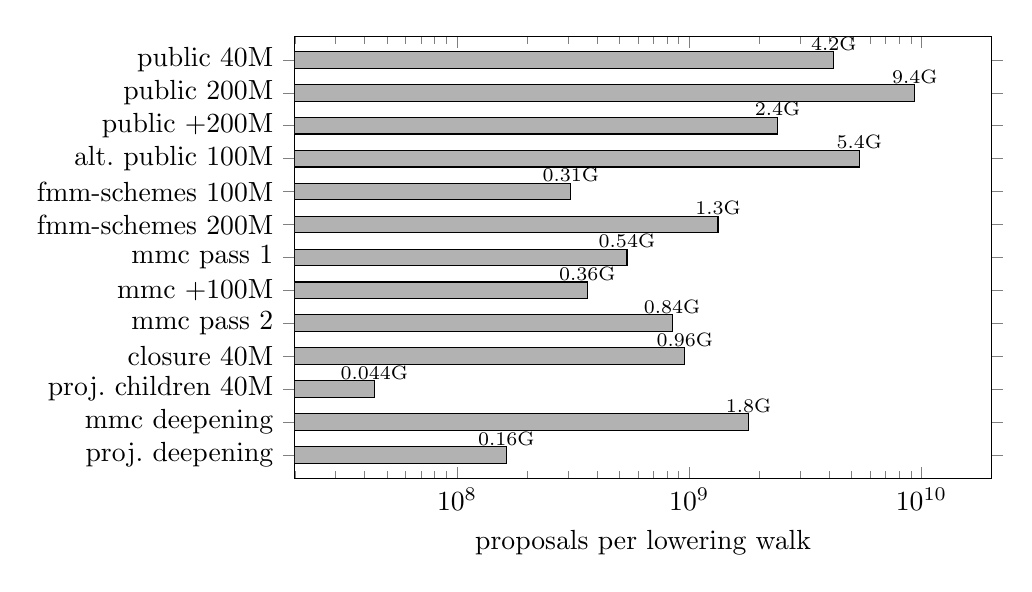
\begin{tikzpicture}
\begin{axis}[xbar,xmode=log,log origin=infty,width=0.86\textwidth,height=7.2cm,
  xmin=2e7,xmax=2e10,bar width=6pt,
  xlabel={proposals per lowering walk},
  symbolic y coords={S1,S2,S3,S4,S5,S6,S7,S8,S9,S10,S11,S12,S13},
  y dir=reverse,ytick=data,enlarge y limits=0.06,
  yticklabels={public 40M,public 200M,public +200M,alt.\ public 100M,fmm-schemes 100M,fmm-schemes 200M,mmc pass 1,mmc +100M,mmc pass 2,closure 40M,proj.\ children 40M,mmc deepening,proj.\ deepening},
  nodes near coords,every node near coord/.append style={font=\scriptsize},
  nodes near coords align={horizontal},
  point meta=explicit symbolic]
\addplot[fill=gray!60] coordinates {(4.19e9,S1) [4.2G] (9.37e9,S2) [9.4G] (2.4e9,S3) [2.4G] (5.4e9,S4) [5.4G] (3.09e8,S5) [0.31G] (1.33e9,S6) [1.3G] (5.39e8,S7) [0.54G] (3.64e8,S8) [0.36G] (8.43e8,S9) [0.84G] (9.57e8,S10) [0.96G] (4.4e7,S11) [0.044G] (1.8e9,S12) [1.8G] (1.63e8,S13) [0.16G]};
\end{axis}
\end{tikzpicture}
\caption{Proposals per lowering walk by stage (\cref{tab:stages}), logarithmic axis. Projection children are cheapest by one to two orders of magnitude, but their lowerings are relative to unreduced seeds.}
\label{fig:yield}
\end{figure}

Three regularities stand out. First, \emph{seeds that are already good rarely improve}: from 629 public integer schemes only six lowered at 40M proposals, every one of them at rank 486 or above; the 367 formats with a seed rank below 486 produced no lowering at all.
In the closure products, no walk from a seed of rank below 1{,}000 (291 walks) lowered, two of 433 below rank 2{,}000 did, against 27 of 261 above; 17 of the 29 lowerings occurred in the 68 walks whose format has a side equal to 11 (25\%, against 1.9\% elsewhere), for a reason we did not investigate.
Second, \emph{unreduced seeds improve almost always}, and this is most of the value of the projection stage for walking, on our reading: it produces seeds with slack.
Third, \emph{the pipeline finds its yield early and near the seed}: of the 228 records with a walk in their lineage (by the index's lineage labels, after correcting one label; walks that did not lower the rank are not counted, and counting them gives 229), the last walk was a 40M walk for 201, a 100M walk for 25 and a 200M walk for two. Most last walks were 40M walks, but 73\% of all walks were.

\subsection{Walk length and continuation}
Longer walks were tried in two ways. \emph{Restarts} walk the same seed again for longer with a different nonce. On the 281 public seeds a five-fold longer walk (200M against 40M) found exactly the six lowerings of the 40M screen and no other; across all 345 seeds walked at more than one length, longer walks produced three lowerings that shorter ones had missed (two from 40M to 100M, one from 100M to 200M), ended lower for 20 seeds, equal for 318 and \emph{higher} for seven.
\emph{Continuations} start from the output of an earlier walk that had lowered the rank, and these do pay: 22 of 80 continuation walks of replayed recipes lowered again (27.5\%), against 7.4\% for the fresh first pass, and 134 of 257 continuations of projection-child walks did (52\%).
Iterated deepening decays quickly: for the replayed-recipe lineage, the lowering rate by round was 8.3\%, 3.3\%, 0\%, 17\%, 0\%, 0\% over 60, 60, 12, 6, 3 and 3 walks.
The reading is that a walk finds what is nearby within the first tens of millions of proposals, and that a further walk from an \emph{improved} scheme has better odds than a longer walk from the same one; we did not test this against random restarts of matched cost.
One observation points the other way: a fresh 5M-proposal walk from the campaign's $24\times31\times32$ witness lowered it (\cref{tab:throughput}), so for that witness the 40M budget stopped short of stagnation; no other large format was tested.

\subsection{Cost of a record}
Dividing the proposals of each log by the records whose last walk came from it gives an upper bound on the price of a record (walks that produced nothing are included in the log's price): between 0.14G and 0.8G proposals for a record whose last walk was a 40M projection-child walk, between 0.45G (closure walks of round 2) and 10G (walks from the fmm-schemes release) for the other classes, and 1.4G on average over the 228 records with a walk if every proposal of the campaign is charged (1.0G if only the logs that ended a record are).
Records reached this way have small margins: for replay-then-walk chains the median margin below the best listed rank is 2 terms.
The large margins of the companion paper come from composition and from certificates produced by earlier stages, not from walks.

\subsection{Negative results}
In addition to those above: 162 alternative public schemes (same rank or one or two above the best) walked for 100M proposals gave three lowerings, each reaching the best public rank and none going below it; the second pass over replayed recipes lowered 38 of 801 at-rank seeds (4.7\%);
after the third round the rank-only closure has no lead left at or below the listed rank (one at 1\%), with the leaves of our scoreboard, which lacked the F2-only schemes of the literature that the companion paper's prior-art check used; and convergence of the projection cascade, which the campaign's notes claimed, is not established: its last pick was under-filled by the defect of \cref{sec:selfref}.

\section{Limitations and threats to validity}\label{sec:limits}

\paragraph{The comparisons are descriptive, not controlled.}
The stages of \cref{tab:stages} differ at once in seed origin, walk length, format range and date, so their yields cannot be attributed to one factor. We did not measure whether directed sampling raises the probability of finding a lower rank compared with uniform sampling, nor whether a longer walk beats several short ones of equal total cost, nor whether the basis rewrite is necessary for any particular record (a later walk might reach the same rank from the plain projection). Every such statement in this paper is a statement about what happened.

\paragraph{Randomness.}
Walk streams are offsets on one full-period linear congruential cycle selected by small, correlated integer nonces, and all seeds of one format within one log share a nonce. We did not test the independence of the streams. Determinism across platforms and compiler versions is untested; only same-machine rebuilds of the same source were replayed, and the binary that ran the first three days was lost with the scratch directory (the sources were unchanged and all 11 first-day walks replay byte for byte with the later build).

\paragraph{Verification.}
Both exactness implementations were written by the same author and share the bit-layout convention. Only 42 of the 244 distinct walks were replayed (\cref{sec:lineage}); closure rows are not rebuilt from leaves by the verifier; five replayed seeds have incomplete leaf provenance; three intermediate witnesses could not be recovered. Exactness of every claimed tensor is established directly and is not affected by any of these.

\paragraph{The campaign had defects that we found and that remain in the data.}
The self-referential child selection (\cref{sec:selfref}) left at least 48 round-3 children unwalked; the deepening queue passed a canonical instead of the file's own orientation for 19 seeds (34 walks) and was stopped in its first round; two rounds of closure materialization crashed at load; seven output files of the alternative-seed walks were overwritten by same-named outputs (none of them was a lowering). The cache-history defect of \cref{sec:cachebug} affected 43 of 1{,}098 replays (relative to the campaign's own pure-mode replays). We report these because they bound what the numbers can support, and because two of them (the cache-history defect and the self-referential selection) were found only when we tried to reproduce or re-derive results.

\paragraph{Comparators and claims.}
The tables are moving and incomplete (\cref{tab:pitfalls}); a result is a triple of scheme, date and revisions, and ``below all listed'' does not mean ``new''. A comparison with the four tables alone overstated novelty: the limited check of the companion paper superseded 87 of the 795 results (32 of the 80 rebuilt ones with F2-only schemes that our own closure lacked as leaves) and matched 112 more by compositions of published schemes and by published rank claims. It was not a complete prior-art audit. Some of the schemes that seed our results are composed from constructions that the project's own notes record as established.

\paragraph{Scope.}
The pipeline finds upper bounds over $\F$ only. It gives no lower bounds and no information about lifting to characteristic zero, and nothing here bears on the exponent of matrix multiplication (the ranks are of small formats and the composition is standard).

\paragraph{Future work.}
The obvious steps are to walk the children that the defect left behind, to run matched-cost comparisons of uniform against directed sampling and of long walks against restarts, to promote the campaign drivers (currently scripts with scratch paths) into the package with parameters, to reduce the residual leaf-provenance gaps, to extend replay to a larger fraction of walks on a cluster, and to re-score against the moving tables at submission time.

\section{Conclusion}
A pipeline built from a directed flip-graph walker, a cheap cross-shape derivation, a rank-only composition closure, careful use of public schemes, and a verification protocol in which every result is checked twice and, wherever possible, re-derived from pinned upstream revisions, produced a large table of upper bounds over $\F$ (reported in the companion paper) at a cost of about $3\times10^{11}$ proposals.
The measured yields say where the effort paid: composition and projection supplied most of the records before the prior-art check, which then superseded or matched 128 of the 203 closure products against 35 of the 288 records with a walk or a projection; walks from already good public schemes supplied very few, and longer walks supplied almost none that the shorter ones had missed.
The engineering lessons are at least as general as the numbers: read the ring from the data and not from the directory; exclude commutative algorithms; treat every table as a dated, moving, field-agnostic bar; make every derivation replayable from a pinned revision; and verify from a clean extraction with empty caches, because a warm cache makes a verifier vacuous.

\section*{Availability}
The search and verification tools are in the package \texttt{tungsten-metaflip} (SPDX: MIT OR Apache-2.0 WITH LLVM-exception; bundled third-party data keeps its own licences, see \texttt{THIRD\_PARTY.md}) of the Tungsten repository \cite{tungsten2026lang}, branch \texttt{main} (the tools of the release are commit \texttt{00ffa04f9}; the sources of these papers, their scripts and the verification logs are in later commits) \todo{push \texttt{main} before submission}.
The tensors of the lineage bundles, the record index, the logs of the release verification and a snapshot of the tools are in a release of \texttt{tungsten-lang/metaflip-archives} (release \texttt{evidence-2026-09-29}), currently private \todo{deposit publicly, e.g.\ on Zenodo, and cite the DOI}.
Each bundle's README gives the exact commands that reproduce its verification; the log of the later Ruby check over all tensors and the closure rebuild log are in the repository (\texttt{papers/verification}).
The FastMatrixMultiplication repository is MIT-licensed, fmm-schemes is CC BY 4.0, the matmulcatalog carries no licence file, and the Lille catalogue is CC BY 3.0 according to its Wikidata record; schemes derived from them keep their attribution, recorded per row.


\section*{Acknowledgements and disclosure}
The search campaign, the tooling and the drafting of this manuscript were assisted by Claude
(Anthropic); the author is responsible for the content.
The pipeline builds on the published work of Kauers and Moosbauer, Arai, Ichikawa and Hukushima,
Moosbauer and Poole, Kauers and Wood, Perminov, Witteveen, Sedoglavic, Lacelle and others cited
below; the schemes that seed or compose our results keep the credit of their authors.
\todo{funding / conflicts-of-interest statement}

\bibliographystyle{plainnat}
\bibliography{refs}

\end{document}
